\section{Background and context}
\label{background}
Currently, there is no official way of encoding the layout of 
computational models in SBML. Software tools wishing to share this 
information have been using the SBML annotation scheme to store this 
information in proprietary form. 

The layout proposal was made in early 2003, since then it has been 
incorporated into libSBML (\cite{Gauges01082006}) and has been used by 
software applications (e.g.: \cite{COPASI}, \cite{sbw}) for SBML Level~2 
and Level~3. 

The overall structure of this proposal reflects design decisions that 
will be detailed in this section. These decisions are mainly based on 
the discussion on the mailing list and during the workshop in St. Louis. 
It was requested that several layouts should be stored in one SBML file. 
And so the layout is stored in a \ListOfLayouts as child of the the 
\Model element instead of direct annotations to the model constituents. 


\begin{center}
\begin{figure}[!h]
\begin{center}
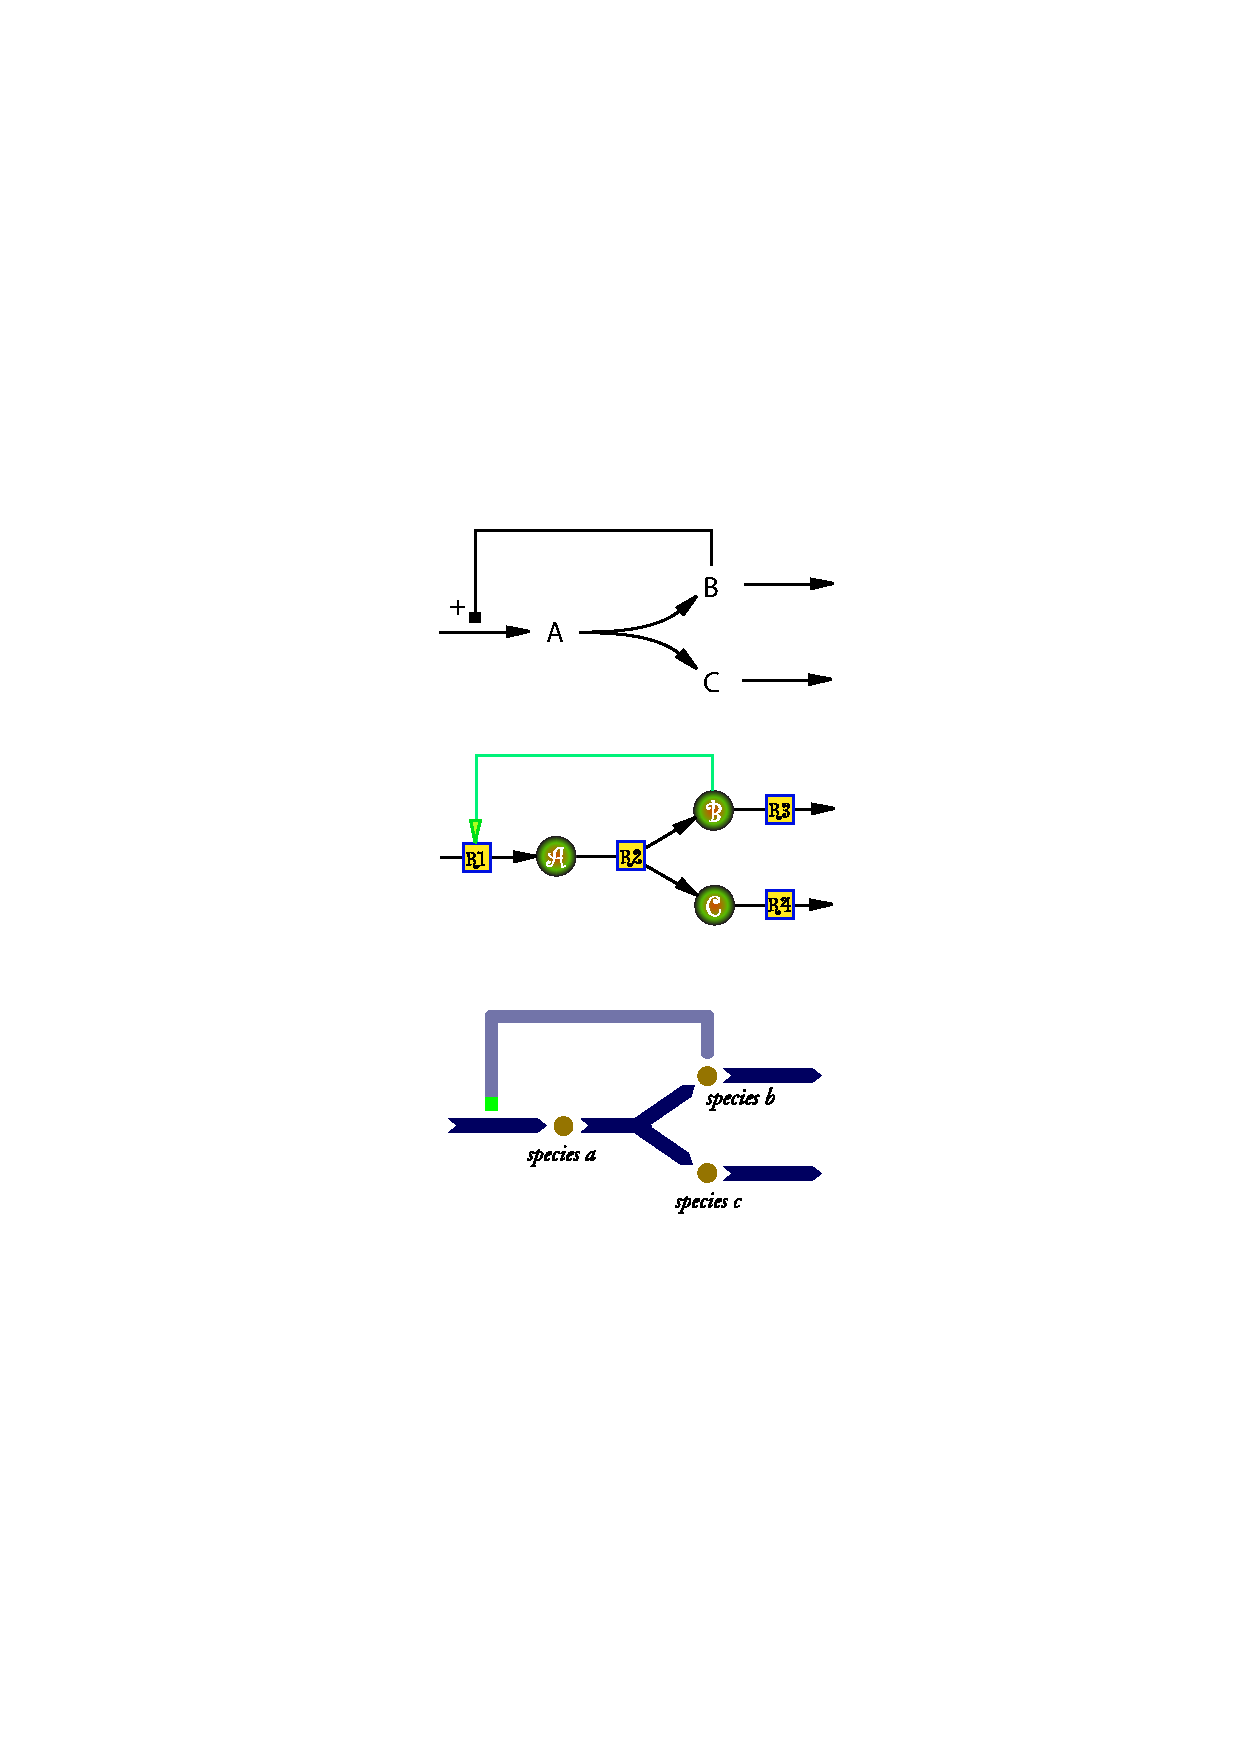
\includegraphics[scale=1]{figures/layout1}
\end{center}
\caption{Illustration of different renderings of the same layout.}
\label{UML:All}
\label{figure:rendering}
\end{figure}
\end{center}

The layout of a reaction network diagram should be described as 
graphical representations of species and reactions (and not as arbitrary 
drawing or graph). This means that existing languages for the 
description of vector drawings (SVG) or general graphs cannot be used. 
While it may seem unnecessary to invent a new language when an existing 
one like SVG could in principle be used to describe the layout of a 
reaction network, there are good reasons to have a language tailored 
specifically for the layout of SBML models. 

Presumably, most programs that will use this SBML extension are 
primarily programs dealing with biochemical models. Internally, they 
will have data structures for species and reactions, so it will be 
natural for them to describe the layout of the reaction network also in 
terms of species and reactions (and not in terms of polygons or 
splines). Thus the \token{layout} object has a similar structure like 
the SBML \token{model} object and contains lists of graphical 
representations of compartments, species, and reactions (called 
\token{compartmentGlyph, speciesGlyph,} and \token{reactionGlyph} 
respectively). Additional layout elements and relationships can be 
represented by using the \token{graphicalObject} and 
\token{generalGlyph} elements. 

Another important question is the level of detail that the description 
should provide. For simplicity, only the layout (i.e., the position of 
the different graphical objects) of the diagram is encoded, not the 
details of how it should be rendered. That is left to the SBML Level~3 
Render package. 

\ref{figure:rendering} illustrates this distinction. All three diagrams 
could be renderings of the same layout and would be described by 
identical SBML files. No information about colors, line styles, fonts, 
etc., is present in the layout description. 

The next question is how the relation between the model and the layout 
should be established. There seems to be consensus that one model 
element can be represented by several layout elements. For example, it 
can be useful to have several representations of one species in the 
layout to avoid crossing lines. This can be accomplished if every layout 
element has a field that refers to the id of a model element. 

There are also cases where a layout element does not correspondent to 
exactly one model element. One example would be if a layout shows a 
simplified version of the model where one reaction in the layout 
corresponds to several reactions and intermediate species in the model. 
This is the reason why the field in the layout elements that refers to 
the model elements is optional, allowing layout objects that do not have 
a specific counterpart in the SBML model. 

The result of all this is a way to describe a graphical layout of a 
reaction network in biochemical terms. This layout can be closely tied 
to the biochemical model. A graphical model editor for example would 
typically create a layout that is closely connected (by a one-to-several 
relation from the model elements to the layout elements) to the model. 

A more general layout design program could also create a layout that is 
not so closely tied to the model, for example, it could create a layout 
that shows a simplified version of the model. 

